Compare las reducciones de Dolittle y Crout con la eliminacion Gausiana con respecto a flop count, requerimientos de almacenamiento y posibilidad de acumulación de productos internos in double precision

\textbf{Solución}

Si definimos cada punto en cuestión:
\begin{itemize}
    \item Flops: Numero de operaciones de multiplicación y división que representan el esfuerzo numérico.
    \item Requerimientos de almacenamiento: Cantidad de almacenamiento necesario para realizar cálculos durante la ejecución del método.
    \item Acumulación de productos internos en precisión doble: Técnica para minimizar la propagación del error.
\end{itemize}

Eliminación Gaussiana.
El numero de flops del algoritmo es:
\begin{itemize}
    \item Bucle interno: "Convertir en cero los elementos abajo del pivote"
    $$\sum_{j=k+1}^{n}1=n-(k+1)\approx n-k$$
    \item Bucle intermedio: 'Calcular los multiplicadores de cada fila'
    $$\sum_{j=k+1}^{n}2+( \text{flops del bucle interno})=\sum_{j=k+1}^{n}2+(n-k)= (2+n-k)(n-k)$$
    $$=(n^2+2n)-2(n+1)k+k^2$$
    \item Bucle exterior: 
    $$\sum_{k=1}^{n-1}n^2+2n.2(n+1)k+k^2$$
    $$=(n^2+2n)\sum_{k=1}^{n-1}1-2(n+1)\sum_{k=1}^{n-1}k+\sum_{k=1}^{n-1}k^2$$
    $$=\frac{n^3}{3} + O(n^3)$$
\end{itemize}
En cuanto a los requerimientos de almacenamiento, el método sobrescribe en la misma matriz $nxn$ los valores obtenidos. Por lo que el método solo necesita almacenar una matriz de tamaño $nxn$ durante su ejecución.

Reduccion Dolittle:
Este método es una forma alternativa para descomponer una matriz en las matrices LU sin tener que utilizar eliminación Gaussiana.
\\ Sea la matriz $A_{nxn}$:
$$A=\begin{bmatrix}
    a_{1,1}&a_{1,2}&...&a_{1,n}\\
    a_{2,1}&a_{2,2}&...&a_{2,n}\\
    ...\\
    a_{n,1}&a_{n,2}&...&a_{n,n}
\end{bmatrix}$$
Asumimos que existen dos matrices $L$ y $U$ tal que:
$$A=LU$$
y las matrices $L$ y $U$ son de la forma:
$$U=\begin{bmatrix}
    u_{1,1}&l_{1,2}&...&u_{1,n}\\
    0&u_{2,2}&...&u_{2,n}\\
    ...\\
    0&0&...&u_{n,n}
\end{bmatrix}$$
$$L=\begin{bmatrix}
    1&0&...&0\\
    l_{2,1}&1&...&0\\
    ...\\
    l_{1,1}&l_{n,2}&...&1
\end{bmatrix}$$
El método de Dolittle calcula los valores $u_{i,j}$ y $l_{i,j}$ con el siguiente algoritmo: \\\\

% Mejor si lo pones en lenguaje Latex...
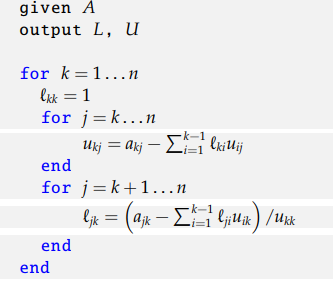
\includegraphics{images/dolittleAlg.PNG}

Si analizamos el algoritmo anterior:
\begin{itemize}
    \item Para el primer bucle (linea 3):
    $$\sum_{j=k}^{n}\sum_{i=1}^{k-1}1=\sum_{j=k}^{n}(k-1)=(k-1)(n-k)$$
    \item Para el segundo bucle interno (linea 9):
    $$\sum_{j=k+1}^{n}\sum_{i=1}^{k-1}1=\sum_{j=k+1}^{n}(k-1)$$
    $$=(n-k-1)(k-1)$$
    \item Para el bucle externo:
     $$\sum_{k=1}^{n}=(k-1)(n-k)+(n-k-1)(k-1)=\sum_{k=1}^{n}1 + k - 2 k^2 - 2 n + 2 k n$$
     Entonces el numero total de FLOPS seria:
     $$=(7 n)/6 - (3 n^2)/2 + n^3/3$$
     
     
\end{itemize}
En cuanto a los requerimientos de almacenamiento de este método, es necesario que durante todo el proceso de calculo se mantengan 3 matrices de tamaño $nxn$ que corresponden a las matrices: $A, L$ y $U$.

Método de Crout:

Este metodo es muy similar al método de Dolittle con la diferencia de que Crout retorna la descomposición LU de la matriz de la forma:
$$U=\begin{bmatrix}
    u_{1,1}&l_{1,2}&...&u_{1,n}\\
    0&u_{2,2}&...&u_{2,n}\\
    ...\\
    0&0&...&u_{n,n}
\end{bmatrix}$$
$$L=\begin{bmatrix}
    1&0&...&0\\
    l_{2,1}&1&...&0\\
    ...\\
    l_{1,1}&l_{n,2}&...&1
\end{bmatrix}$$
mientras que Crout retorna:
$$U=\begin{bmatrix}
    1&l_{1,2}&...&u_{1,n}\\
    0&1&...&u_{2,n}\\
    ...\\
    0&0&...&1
\end{bmatrix}$$
$$L=\begin{bmatrix}
    l_{1,1}&0&...&0\\
    l_{2,1}&l_{2,2}&...&0\\
    ...\\
    l_{1,1}&l_{n,2}&...&l_{n,n}
\end{bmatrix}$$
El conteo de flops del algoritmo de Crout es muy similar al metodo de Dolittle. Es decir $O(n^3/3)$.
En cuanto a los requerimientos de almacenamiento. Es necesario mantener 3 matrices $n$x$n$ que corresponden a las matrices $A,L$ y $U$.

Por lo tanto al comparar los 3 métodos tendríamos que:

\begin{itemize}
    \item Flops: Los 3 metodos realizan una cantidad total de FLOPS parecidas de orden $O(n^3/3)$.
    \item Requerimientos de almacenamiento: La eliminacion de Gauss utiliza la matriz original $n$x$n$. Tanto Dolittle como Crout utilizan 2 matrices $n$x$n$ que corresponden a las matrices $L$ y U, ademas de la matriz original.
    \item Acumulacion de productos internos en precision doble: Crout permite la acumulacion de productos internos en doble precision. Gauss no permite esto 
    
\end{itemize}